\qrchapterstar{https://forgottenpillar.com/rsc/en-fp-appendix}{Appendix} \label{chap:appendix}


\qrchapterstar{https://forgottenpillar.com/rsc/en-fp-appendix}{Apéndice} \label{chap:appendix}


\addcontentsline{toc}{chapter}{Appendix}


\addcontentsline{toc}{chapter}{Apéndice}


\section*{The Fundamental Principles 1889}


\section*{Los Principios Fundamentales 1889}


As elsewhere stated, Seventh-day Adventists have no creed but the Bible; but they hold to certain well-defined points of faith for which they feel prepared to give a reason “to every man that asketh” them. The following propositions may be taken as a summary of the principal features of their religious faith, upon which there is, so far as we know, entire unanimity throughout the body. They believe,—


Como ya se ha dicho, los Adventistas del Séptimo Día no tienen más credo que la Biblia; pero sostienen ciertos puntos de fe bien definidos para los cuales se sienten preparados para dar una razón “a todo hombre que se los pida”. Las siguientes proposiciones pueden tomarse como un resumen de los principales rasgos de su fe religiosa, sobre los cuales hay, por lo que sabemos, total unanimidad en todo el cuerpo. Ellos creen,—


\lettrine{I.} That there is one God, a personal, spiritual being, the creator of all things, omnipotent, omniscient, and eternal; infinite in wisdom, holiness, justice, goodness, truth, and mercy; unchangeable, and everywhere present by his representative, the Holy Spirit. Psalm 139:7.


\lettrine{I.} Que hay un solo Dios, un ser personal y espiritual, creador de todas las cosas, omnipotente, omnisciente y eterno; infinito en sabiduría, santidad, justicia, bondad, verdad y misericordia; inmutable y presente en todas partes por medio de su representante, el Espíritu Santo. Salmo 139:7.


\lettrine{II.} That there is one Lord Jesus Christ, the Son of the Eternal Father, the one by whom he created all things, and by whom they do consist; that he took on him the nature of the seed of Abraham for the redemption of our fallen race; that he dwelt among men, full of grace and truth, lived our example, died our sacrifice, was raised for our justification, ascended on high to be our only mediator in the sanctuary in heaven, where, through the merits of his shed blood, he secures the pardon and forgiveness of the sins of all those who penitently come to him; and as the closing portion of his work as priest, before he takes his throne as king, he will make the great atonement for the sins of all such, and their sins will then be blotted out (Acts 3:19) and borne away from the sanctuary, as shown in the service of the Levitical priesthood, which foreshadowed and prefigured the ministry of our Lord in heaven. See Leviticus 16; Hebrews 8:4, 5; 9:6, 7; etc.


\lettrine{II.} Que hay un solo Señor Jesucristo, el Hijo del Padre Eterno, aquel por quien él creó todas las cosas, y por quien consisten; que tomó sobre sí la naturaleza de la simiente de Abraham para la redención de nuestra raza caída; que habitó entre los hombres, lleno de gracia y de verdad, vivió nuestro ejemplo, murió nuestro sacrificio, fue resucitado para nuestra justificación, ascendió a lo alto para ser nuestro único mediador en el santuario del cielo, donde, por los méritos de su sangre derramada, asegura el perdón y la remisión de los pecados de todos aquellos que acuden a él penitentemente; y como la porción final de su trabajo como sacerdote, antes de tomar su trono como rey, hará la gran expiación por los pecados de todos ellos, y sus pecados serán entonces borrados (Hechos 3:19) y serán retirados del santuario, como se muestra en el servicio del sacerdocio levítico, que anunciaba y prefiguraba el ministerio de nuestro Señor en el cielo. Véase Levítico 16; Hebreos 8:4, 5; 9:6, 7; etc.


\lettrine{III.} That the Holy Scriptures of the Old and New Testaments were given by inspiration of God, contain a full revelation of his will to man, and are the only infallible rule of faith and practice.


\lettrine{III.} Que las Sagradas Escrituras del Antiguo y del Nuevo Testamento fueron dadas por inspiración de Dios, contienen una revelación completa de su voluntad al hombre y son la única regla infalible de fe y práctica.


\lettrine{IV.} That baptism is an ordinance of the Christian church, to follow faith and repentance,—an ordinance by which we commemorate the resurrection of Christ, as by this act we show our faith in his burial and resurrection, and through that, in the resurrection of all the saints at the last day; and that no other mode more fitly represents these facts than that which the Scriptures prescribe, namely, immersion. Romans 6:3-5; Colossians 2:12.


\lettrine{IV.} Que el bautismo es una ordenanza de la iglesia cristiana, que debe seguir a la fe y al arrepentimiento,—una ordenanza por la que conmemoramos la resurrección de Cristo, ya que por este acto mostramos nuestra fe en su sepultura y resurrección, y por medio de ella, en la resurrección de todos los santos en el último día; y que ningún otro modo representa más adecuadamente estos hechos que el que prescriben las Escrituras, es decir, por inmersión. Romanos 6:3-5; Colosenses 2:12.


\lettrine{V.} That the new birth comprises the entire change necessary to fit us for the kingdom of God, and consists of two parts; First, a moral change wrought by conversion and a Christian life (John 3:3, 5); second, a physical change at the second coming of Christ, whereby, if dead, we are raised incorruptible, and if living, are changed to immortality in a moment, in the twinkling of an eye. Luke 20:36; 1 Corinthians 15:51, 52.


\lettrine{V.} Que el nuevo nacimiento abarca todo el cambio necesario para capacitarnos para el reino de Dios, y consta de dos partes: primero, un cambio moral efectuado por la conversión y una vida cristiana (Juan 3:3, 5); segundo, un cambio físico en la segunda venida de Cristo, por el cual, si estamos muertos, somos resucitados incorruptibles, y si estamos vivos, somos cambiados a inmortalidad en un momento, en un abrir y cerrar de ojos. Lucas 20:36; 1 Corintios 15:51, 52.


\lettrine{VI.} That prophecy is a part of God’s revelation to man; that it is included in that Scripture which is profitable for instruction (2 Timothy 3:16); that it is designed for us and our children (Deuteronomy 29:29); that so far from being enshrouded in impenetrable mystery, it is that which especially constitutes the word of God a lamp to our feet and a light to our path (Psalm 119:105; 2 Peter 1:19); that a blessing is pronounced upon those who study it (Revelation 1:1-3); and that, consequently, it is to be understood by the people of God sufficiently to show them their position in the world’s history and the special duties required at their hands.


\lettrine{VI.} Que la profecía es una parte de la revelación de Dios al hombre; que está incluida en esa escritura que es útil para la instrucción (2 Timoteo 3:16); que está diseñada para nosotros y nuestros hijos (Deuteronomio 29:29); que lejos de estar envuelta en un misterio impenetrable, es eso que especialmente constituye la palabra de Dios como una lámpara para nuestros pies y una luz para nuestro camino (Salmo 119:105; 2 Pedro 1:19); que se pronuncia una bendición sobre los que la estudian (Apocalipsis 1:1-3); y que, en consecuencia, debe ser comprendida por el pueblo de Dios lo suficiente como para mostrarle su posición en la historia del mundo y los deberes especiales requeridos en sus manos.


\lettrine{VII.} That the world’s history from specified dates in the past, the rise and fall of empires, and the chronological succession of events down to the setting up of God’s everlasting kingdom, are outlined in numerous great chains of prophecy; and that these prophecies are now all fulfilled except the closing scenes.


\lettrine{VII.} Que la historia del mundo desde fechas específicas en el pasado, el surgimiento y la caída de imperios, y la sucesión cronológica de acontecimientos hasta el establecimiento del reino eterno de Dios, están delineados en numerosas grandes cadenas de profecía; y que estas profecías están ahora todas cumplidas, excepto las escenas finales.


\lettrine{VIII.} That the doctrine of the world’s conversion and a temporal millennium is a fable of these last days, calculated to lull men into a state of carnal security, and cause them to be overtaken by the great day of the Lord as by a thief in the night (1 Thessalonians 5:3); that the second coming of Christ is to precede, not follow, the millennium; for until the Lord appears, the papal power, with all its abominations, is to continue (2 Thessalonians 2:8), the wheat and tares grow together (Matthew 13:29, 30, 39), and evil men and seducers wax worse and worse, as the word of God declares. 2 Timothy 3:1, 13.


\lettrine{VIII.} Que la doctrina de la conversión del mundo y de un milenio temporal es una fábula de estos últimos días, calculada para adormecer a los hombres en un estado de seguridad carnal, y causar que sean sorprendidos por el gran día del Señor como por un ladrón en la noche (1 Tesalonicenses 5:3); que la segunda venida de Cristo ha de preceder, no seguir, al milenio; porque hasta que aparezca el Señor, el poder papal, con todas sus abominaciones, ha de continuar (2 Tesalonicenses 2:8), el trigo y la cizaña crecen juntos (Mateo 13:29, 30, 39), y los hombres malos y los seductores empeoran cada vez más, como declara la palabra de Dios. 2 Timoteo 3:1, 13.


\lettrine{IX.} That the mistake of Adventists in 1844 pertained to the nature of the event then to transpire, not to the time; that no prophetic period is given to reach to the second advent, but that the longest one, the two thousand and three hundred days of Daniel 8:14, terminated in 1844, and brought us to an event called the cleansing of the sanctuary.


\lettrine{IX.} Que el error de los adventistas en 1844 se refería a la naturaleza del acontecimiento que iba a ocurrir entonces, no al tiempo; que ningún período profético está determinado a llegar al segundo advenimiento, sino que el más largo, los dos mil trescientos días de Daniel 8:14, terminó en 1844, y nos trajo a un acontecimiento llamado la purificación del santuario.


\lettrine{X.} That the sanctuary of the new covenant is the tabernacle of God in heaven, of which Paul speaks in Hebrews 8 and onward, and of which our Lord, as great high priest, is minister; that this sanctuary is the antitype of the Mosaic tabernacle, and that the priestly work of our Lord, connected therewith, is the antitype of the work of the Jewish priests of the former dispensation (Hebrews 8:1-5, etc.); that this, and not the earth, is the sanctuary to be cleansed at the end of the two thousand and three hundred days, what is termed its cleansing being in this case, as in the type, simply the entrance of the high priest into the most holy place, to finish the round of service connected therewith, by making the atonement and removing from the sanctuary the sins which had been transferred to it by means of the ministration in the first apartment (Leviticus 16; Hebrews 9:22, 23); and that this work in the antitype, beginning in 1844, consists in actually blotting out the sins of believers (Acts 3:19), and occupies a brief but indefinite space of time, at the conclusion of which the work of mercy for the world will be finished, and the second advent of Christ will take place.


\lettrine{X.} Que el santuario del nuevo pacto es el tabernáculo de Dios en el cielo, del cual habla Pablo en Hebreos 8 y en adelante, y del cual nuestro Señor, como gran sumo sacerdote, es ministro; que este santuario es el antitipo del tabernáculo mosaico, y que la obra sacerdotal de nuestro Señor, relacionada con él, es el antitipo de la obra de los sacerdotes judíos de la dispensación anterior (Hebreos 8:1-5, etc.); que éste, y no la tierra, es el santuario que había de ser purificado al final de los dos mil trescientos días, siendo lo que se denomina su purificación en este caso, como en el tipo, simplemente la entrada del sumo sacerdote en el lugar santísimo, para terminar la ronda de servicio relacionada con él, haciendo la expiación y quitando del santuario los pecados que habían sido transferidos a él por medio de la ministración en el primer departamento (Levítico 16; Hebreos 9:22, 23); y que esta obra en el antitipo, que comienza en 1844, consiste en borrar realmente los pecados de los creyentes (Hechos 3:19), y ocupa un espacio de tiempo breve pero indefinido, al final del cual la obra de misericordia para el mundo estará terminada, y tendrá lugar el segundo advenimiento de Cristo.


\lettrine{XI.} That God’s moral requirements are the same upon all men in all dispensations; that these are summarily contained in the commandments spoken by Jehovah from Sinai, engraven on the tables of stone, and deposited in the ark, which was in consequence called the “ark of the covenant,” or testament (Numbers 10:33; Hebrews 9:4, etc.); that this law is immutable and perpetual, being a transcript of the tables deposited in the ark in the true sanctuary on high, which is also, for the same reason, called the ark of God’s testament; for under the sounding of the seventh trumpet we are told that “the temple of God was opened in heaven, and there was seen in his temple the ark of his testament.” Revelation 11:19.


\lettrine{XI.} Que los requisitos morales de Dios son los mismos para todos los hombres en todas las dispensaciones; que éstos están contenidos sumariamente en los mandamientos pronunciados por Jehová desde el Sinaí, grabados en las tablas de piedra y depositados en el arca, la cual fue llamada en consecuencia “arca del pacto” o testamento (Números 10:33; Hebreos 9:4, etc.); que esta ley es inmutable y perpetua, siendo una transcripción de las tablas depositadas en el arca en el verdadero santuario en lo alto, que también es, por la misma razón, llamada el arca del testamento de Dios; porque bajo el sonido de la séptima trompeta se nos dice que “el templo de Dios fue abierto en el cielo, y se vio en su templo el arca de su testamento”. Apocalipsis 11:19.


\lettrine{XII.} That the fourth commandment of this law requires that we devote the seventh day of each week, commonly called Saturday, to abstinence from our own labor, and to the performance of sacred and religious duties; that this is the only weekly Sabbath known to the Bible, being the day that was set apart before Paradise was lost (Genesis 2:2, 3), and which will be observed in Paradise restored (Isaiah 66:22, 23); that the facts upon which the Sabbath institution is based confine it to the seventh day, as they are not true of any other day; and that the terms Jewish Sabbath, as applied to the seventh day, and Christian Sabbath, as applied to the first day of the week, are names of human invention, unscriptural in fact, and false in meaning.


\lettrine{XII.} Que el cuarto mandamiento de esta ley requiere que dediquemos el séptimo día de cada semana, comúnmente llamado sábado, a la abstinencia de nuestro propio trabajo y al desempeño de deberes sagrados y religiosos; que éste es el único sábado semanal conocido por la Biblia, siendo el día que fue apartado antes de que se perdiera el paraíso (Génesis 2:2, 3), y el cual será observado en el paraíso restaurado (Isaías 66:22, 23); que los hechos en los que se basa la institución del sábado lo limitan al séptimo día, ya que no son ciertos para ningún otro día; y que los términos sábado judío, aplicado al séptimo día, y sábado cristiano, aplicado al primer día de la semana, son nombres de invención humana, no bíblicos de hecho, y falsos en significado.


\lettrine{XIII.} That as the man of sin, the papacy, has thought to change times and laws (the law of God, Daniel 7:25), and has misled almost all Christendom in regard to the fourth commandment, we find a prophecy of a reform in this respect to be wrought among believers just before the coming of Christ. Isaiah 56:1, 2; 1 Peter 1:5; Revelation 14:12, etc.


\lettrine{XIII.} Que como el hombre de pecado, el papado, ha pensado en cambiar los tiempos y las leyes (la ley de Dios, Daniel 7:25), y ha engañado a casi toda la cristiandad con respecto al cuarto mandamiento, encontramos una profecía de una reforma a este respecto que se llevará a cabo entre los creyentes justo antes de la venida de Cristo. Isaías 56:1, 2; 1 Pedro 1:5; Apocalipsis 14:12, etc.


\lettrine{XIV.} That the followers of Christ should be a peculiar people, not following the maxims, nor conforming to the ways, of the world; not loving its pleasures nor countenancing its follies; inasmuch as the apostle says that “whosoever therefore will be” in this sense, “a friend of the world, is the enemy of God” (James 4:4); and Christ says that we cannot have two masters, or, at the same time, serve God and mammon. Matthew 6:24.


\lettrine{XIV.} Que los seguidores de Cristo deben ser un pueblo peculiar, que no siga las máximas ni se ajuste a los caminos del mundo; que no ame sus placeres ni tolere sus locuras; ya que el apóstol dice que “cualquiera, pues, que quiera ser” en este sentido, “amigo del mundo, se constituye enemigo de Dios” (Santiago 4:4); y Cristo dice que no podemos tener dos amos, o, al mismo tiempo, servir a Dios y a las riquezas. Mateo 6:24.


\lettrine{XV.} That the Scriptures insist upon plainness and modesty of attire as a prominent mark of discipleship in those who profess to be the followers of Him who was, “meek and lowly in heart,” that the wearing of gold, pearls, and costly array, or anything designed merely to adorn the person and foster the pride of the natural heart, is to be discarded, according to such scriptures as 1 Timothy 2:9, 10; 1 Peter 3:3, 4.


\lettrine{XV.} Que las escrituras insisten en la sencillez y la modestia de la vestimenta como una marca prominente del discipulado en aquellos que profesan ser los seguidores de Aquel que fue “manso y humilde de corazón”, que el vestir de oro, perlas, y ropa costosa, o cualquier cosa diseñada meramente para adornar la persona y fomentar el orgullo del corazón natural, debe ser desechado, de acuerdo con escrituras tales como 1 Timoteo 2:9, 10; 1 Pedro 3:3, 4.


\lettrine{XVI.} That means for the support of evangelical work among men should be contributed from love to God and love of souls, not raised by church lotteries, or occasions designed to contribute to the fun-loving, appetite-indulging propensities of the sinner, such as fairs, festivals, oyster suppers, tea, broom, donkey, and crazy socials, etc., which are a disgrace to the professed church of Christ; that the proportion of one’s income required in former dispensation can be no less under the gospel; that it is the same as Abraham (whose children we are, if we are Christ’s, Galatians 3:29) paid to Melchisedec (type of Christ) when he gave him a tenth of all (Hebrews 7:1-4); the title is the Lord’s (Leviticus 27:30); and this tenth of one’s income is also to be supplemented by offerings from those who are able, for the support of the gospel. 2 Corinthians 9:6; Malachi 3:8, 10.


\lettrine{XVI.} Que los medios para el sostenimiento de la obra evangélica entre los hombres deben ser aportados por amor a Dios y por amor a las almas, y no recaudados por loterías de la iglesia, o por ocasiones diseñadas para contribuir a las propensiones amantes de la diversión y complacientes del apetito del pecador, tales como ferias, festivales, cenas de ostras, fiestas del té, de la escoba, del burro y de la locura, etc., que son una vergüenza para la profesa iglesia de Cristo; que la proporción de los ingresos de uno requerida en la dispensación anterior no puede ser menor bajo el evangelio; que es lo mismo que Abraham (cuyos hijos somos, si somos de Cristo, Gálatas 3:29) pagó a Melquisedec (tipo de Cristo) cuando le dio la décima parte de todo (Hebreos 7:1-4); el diezmo es del Señor (Levítico 27:30); y esta décima parte de los ingresos de uno también debe ser complementada con ofrendas de aquellos que pueden, para el apoyo del evangelio. 2 Corintios 9:6; Malaquías 3:8, 10.


\lettrine{XVII.} That as the natural or carnal heart is at enmity with God and his law, this enmity can be subdued only by a radical transformation of the affections, the exchange of unholy for holy principles; that this transformation follows repentance and faith, is the special work of the Holy Spirit, and constitutes regeneration, or conversion.


\lettrine{XVII.} Que como el corazón natural o carnal está en enemistad con Dios y su ley, esta enemistad sólo puede ser subyugada por una transformación radical de los afectos, el cambio de principios impíos por santos; que esta transformación sigue al arrepentimiento y a la fe, es la obra especial del Espíritu Santo y constituye la regeneración o conversión.


\lettrine{XVIII.} That as all have violated the law of God, and cannot of themselves render obedience to his just requirements, we are dependent on Christ, first, for justification from our past offenses, and, secondly, for grace whereby to render acceptable obedience to his holy law in time to come.


\lettrine{XVIII.} Que como todos han violado la ley de Dios, y no pueden por sí mismos rendir obediencia a sus justos requerimientos, dependemos de Cristo, primero, para la justificación de nuestras ofensas pasadas, y, segundo, para la gracia que nos permita rendir obediencia aceptable a su santa ley en el tiempo venidero.


\lettrine{XIX.} That the Spirit of God was promised to manifest itself in the church through certain gifts, enumerated especially in 1 Corinthians 12 and Ephesians 4; that these gifts are not designed to supersede, or take the place of, the Bible, which is sufficient to make us wise unto salvation, any more than the Bible can take the place of the Holy Spirit; that, in specifying the various channels of its operation, that Spirit has simply made provision for its own existence and presence with the people of God to the end of time, to lead to an understanding of that word which it had inspired, to convince of sin, and to work a transformation in the heart and life; and that those who deny to the Spirit its place and operation, do plainly deny that part of the Bible which assigns to it this work and position.


\lettrine{XIX.} Que el Espíritu de Dios fue prometido para manifestarse en la iglesia a través de ciertos dones, enumerados especialmente en 1 Corintios 12 y Efesios 4; que estos dones no están diseñados para sustituir o tomar el lugar de la Biblia, la cual es suficiente para hacernos sabios para la salvación, así como tampoco la Biblia puede tomar el lugar del Espíritu Santo; que, al especificar los diversos canales de su operación, ese Espíritu simplemente ha hecho provisión para su propia existencia y presencia con el pueblo de Dios hasta el fin del tiempo, para llevar a la comprensión de esa palabra que había inspirado, para convencer del pecado, y para obrar una transformación en el corazón y la vida; y que aquellos que niegan al Espíritu su lugar y operación, niegan claramente la parte de la Biblia que le asigna esta obra y posición.


\lettrine{XX.} That God, in accordance with his uniform dealings with the race, sends forth a proclamation of the approach of the second advent of Christ; and that this work is symbolized by the three messages of Revelation 14, the last one bringing to view the work of reform on the law of God, that his people may acquire a complete readiness for that event.


\lettrine{XX.} Que Dios, de acuerdo con sus tratos uniformes con la raza, envía una proclamación de la aproximación del segundo advenimiento de Cristo; y que esta obra está simbolizada por los tres mensajes de Apocalipsis 14, el último de los cuales trae a la vista la obra de reforma sobre la ley de Dios, para que su pueblo adquiera una completa preparación para ese acontecimiento.


\lettrine{XXI.} That the time of the cleansing of the sanctuary (See proposition X.), synchronizing with the time of the proclamation of the third message (Revelation 14:9, 10), is a time of investigative judgment, first, with reference to the dead, and secondly, at the close of probation, with reference to the living, to determine who of the myriads now sleeping in the dust of the earth are worthy of a part in the first resurrection, and who of its living multitudes are worthy of translation,—points which must be determined before the Lord appears.


\lettrine{XXI.} Que el tiempo de la purificación del santuario (véase la proposición X.), sincronizando con el tiempo de la proclamación del tercer mensaje (Apocalipsis 14:9, 10), es un tiempo de juicio investigador, primero, con referencia a los muertos, y segundo, al final del tiempo de gracia, con referencia a los vivos, para determinar quiénes de las miriadas que ahora duermen en el polvo de la tierra son dignos de una parte en la primera resurrección, y quiénes de sus multitudes vivas son dignos de ser trasladados—puntos que deben ser determinados antes de que el Señor aparezca.


\lettrine{XXII.} That the grave, whether we all tend, expressed by the Hebrew word sheol and the Greek word hades, is a place, or condition, in which there is no work, device, wisdom, nor knowledge. Ecclesiastes 9:10.


\lettrine{XXII.} Que el sepulcro, al que todos tendemos, expresado por la palabra hebrea sheol y la griega hades, es un lugar, o condición, en el que no hay obra, trabajo, sabiduría ni conocimiento. Eclesiastés 9:10.


\lettrine{XXIII.} That the state to which we are reduced by death is one of silence, inactivity, and entire unconsciousness. Psalm 146:4; Ecclesiastes 9:5, 6; Daniel 12:2.


\lettrine{XXIII.} Que el estado al que somos reducidos por la muerte es uno de silencio, inactividad y total inconsciencia. Salmo 146:4; Eclesiastés 9:5, 6; Daniel 12:2.


\lettrine{XXIV.} That out of this prison-house of the grave, mankind are to be brought by a bodily resurrection; the righteous having part in the first resurrection, which takes place at the second coming of Christ; the wicked, in the second resurrection, which takes place in a thousand years thereafter. Revelation 20:4-6.


\lettrine{XXIV.} Que fuera de esta prisión de la tumba, la humanidad será sacada por una resurrección corporal; los justos teniendo parte en la primera resurrección, que tiene lugar en la segunda venida de Cristo; los impíos, en la segunda resurrección, que tiene lugar mil años después. Apocalipsis 20:4-6.


\lettrine{XXV.} That at the last trump, the living righteous are to be changed in a moment, in the twinkling of an eye, and with the risen righteous are to be caught up to meet the Lord in the air, so forever to be with the Lord. 1 Thessalonians 4:16, 17; 1 Corinthians 15:51, 52.


\lettrine{XXV.} Que a la última trompeta, los justos vivos serán cambiados en un momento, en un abrir y cerrar de ojos, y con los justos resucitados serán arrebatados para encontrarse con el Señor en el aire, para estar siempre así con el Señor. 1 Tesalonicenses 4:16, 17; 1 Corintios 15:51, 52.


\lettrine{XXVI.} That these immortalized ones are then taken to heaven, to the New Jerusalem, the Father’s house, in which there are many mansions (John 14:1-3), where they reign with Christ a thousand years, judging the world and fallen angels, that is, apportioning the punishment to be executed upon them at the close of the one thousand years (Revelation 20:4; 1 Corinthians 6:2, 3); that during this time the earth lies in a desolate and chaotic condition (Jeremiah 4:23-27), described, as in the beginning, by the Greek term abussos— “bottom-less pit” (Septuagint of Genesis 1:2); and that here Satan is confined during the thousand years (Revelation 20:1, 2), and here finally destroyed (Revelation 20:10; Malachi 4:1); the theater of the ruin he has wrought in the universe being appropriately made, for a time, his gloomy prison-house, and then the place of his final execution.


\lettrine{XXVI.} Que estos inmortalizados son entonces llevados al cielo, a la Nueva Jerusalén, la casa del Padre, en la que hay muchas mansiones (Juan 14:1-3), donde reinan con Cristo mil años, juzgando al mundo y a los ángeles caídos, es decir, impartiendo el castigo que se ejecutará sobre ellos al final de los mil años (Apocalipsis 20:4; 1 Corintios 6:2, 3); que durante este tiempo la tierra yace en una condición desolada y caótica (Jeremías 4:23-27), descrita, como en el principio, por el término griego abussos—“pozo sin fondo” (Septuaginta de Génesis 1:2); y que aquí Satanás es confinado durante los mil años (Apocalipsis 20:1, 2), y aquí es finalmente destruido (Apocalipsis 20:10; Malaquías 4:1); el teatro de la ruina que él ha causado en el universo es apropiadamente hecho, por un tiempo, su sombría prisión, y luego el lugar de su ejecución final.


\lettrine{XXVII.} That at the end of the thousand years the Lord descends with his people and the New Jerusalem (Revelation 21:2), the wicked dead are raised, and come up on the surface of the yet unrenewed earth, and gather about the city, the camp of the saints (Revelation 20:9), and fire comes down from God out of heaven and devours them. They are then consumed, root and branch (Malachi 4:1), becoming as though they had not been. Obadiah 15, 16. In this everlasting destruction from the presence of the Lord (2 Thessalonians 1:9), the wicked meet the “everlasting punishment” threatened against them (Matthew 25:46), which is everlasting death. Romans 6:23; Revelation 20:14, 15. This is the perdition of ungodly men, the fire which consumes them being the fire for which “the heavens and the earth, which are now,... are kept in store.” which shall melt even the elements with its intensity, and purge the earth from the deepest stains of the curse of sin. 2 Peter 3:7-12.


\lettrine{XXVII.} Que al final de los mil años el Señor desciende con su pueblo y la Nueva Jerusalén (Apocalipsis 21:2), los impíos muertos son resucitados y suben a la superficie de la tierra aún no renovada, y se reúnen alrededor de la ciudad, el campamento de los santos (Apocalipsis 20:9), y fuego desciende de Dios desde el cielo y los devora. Entonces son consumidos, raíz y rama (Malaquías 4:1), quedando como si no hubieran existido. Abdías 15, 16. En esta destrucción eterna de la presencia del Señor (2 Tesalonicenses 1:9), los impíos reciben el “castigo eterno” amenazado contra ellos (Mateo 25:46), que es la muerte eterna. Romanos 6:23; Apocalipsis 20:14, 15. Esta es la perdición de los hombres impíos, siendo el fuego que los consume el fuego para el cual “los cielos y la tierra, que son ahora,... están guardados”, que derretirá hasta los elementos con su intensidad, y purificará la tierra de las manchas más profundas de la maldición del pecado. 2 Pedro 3:7-12.


\lettrine{XXVIII.} That new heavens and a new earth shall spring by the power of God from the ashes of the old, and this renewed earth, with the New Jerusalem for its metropolis and capital, shall be the eternal inheritance of the saints, the place where the righteous shall evermore dwell. 2 Peter 3:13; Psalm 37:11, 29; Matthew 5:5.


\lettrine{XXVIII.} Que nuevos cielos y una nueva tierra brotarán por el poder de Dios de las cenizas de los antiguos, y esta tierra renovada, con la Nueva Jerusalén como metrópoli y capital, será la herencia eterna de los santos, el lugar donde los justos habitarán para siempre. 2 Pedro 3:13; Salmo 37:11, 29; Mateo 5:5.


\section*{Fundamental Principles - Timeline} \label{appendix:timeline}


\section*{Principios Fundamentales - Cronología} \label{appendix:timeline}


The following is a list of some appearances of the Declaration of Fundamental Principles in our publications. All links are accessible at \href{https://notefp.link/fp-timeline}{https://notefp.link/fp-timeline}.


La siguiente es una lista de algunas apariciones de la Declaración de los Principios Fundamentales en nuestras publicaciones. Todos los enlaces son accesibles en \href{https://notefp.link/fp-timeline}{https://notefp.link/fp-timeline}.


\leftsubsection{1872 - The first appearance}


\leftsubsection{1872 - La primera aparición}


\textit{“A Declaration of the Fundamental Principles Taught and Practiced by Seventh-day Adventists}” - printed as a pamphlet (\href{https://adventistdigitallibrary.org/islandora/object/adl:366607?link_only=true}{original scan} \href{https://forgotten-pillar.s3.us-east-2.amazonaws.com/A+declaration+of+the+fundamental+principles+taught+and+practiced+by+the+Seventh-day+Adventists++.pdf}{*}). They appeared anonymous, presented as a short public synopsis of what Seventh-day Adventists believe.


\textit{“Declaración de los Principios Fundamentales, Enseñados y Practicados por los Adventistas del Séptimo Día”} - impreso como un folleto (\href{https://adventistdigitallibrary.org/islandora/object/adl:366607?link_only=true}{escaneo original} \href{https://forgotten-pillar.s3.us-east-2.amazonaws.com/A+declaration+of+the+fundamental+principles+taught+and+practiced+by+the+Seventh-day+Adventists++.pdf}{*}). Aparecieron de forma anónima, presentados como un breve resumen público de lo que creen los Adventistas del Séptimo Día.


\leftsubsection{1874 - The Signs of the Times}


\leftsubsection{1874 - The Signs of the Times}


Original scan: \href{https://adventistdigitallibrary.org/adl-364148/signs-times-june-4-1874}{ST June 4, 1874, p.3.} \href{https://forgotten-pillar.s3.us-east-2.amazonaws.com/Signs+of+the+Times+_+June+4%2C+1874++.pdf}{*} James White stood behind the declaration as a main editor of the Signs of the Times at that time.


Escaneo original: \href{https://adventistdigitallibrary.org/adl-364148/signs-times-june-4-1874}{ST 4 de junio de 1874, p.3.} \href{https://forgotten-pillar.s3.us-east-2.amazonaws.com/Signs+of+the+Times+_+June+4%2C+1874++.pdf}{*} James White respaldó la declaración como editor principal de Signs of the Times en ese momento.


\leftsubsection{1874 - The Advent Review and Herald of the Sabbath}


\leftsubsection{1874 - The Advent Review and Herald of the Sabbath}


Original scan: \href{https://documents.adventistarchives.org/Periodicals/RH/RH18741124-V44-22.pdf}{RH November 24, 1874, p.171} \href{https://forgotten-pillar.s3.us-east-2.amazonaws.com/RH18741124-V44-22.pdf}{*} Uriah Smith signed the declaration as the main editor of the Review and Herald of the Sabbath periodical at that time.


Escaneo original: \href{https://documents.adventistarchives.org/Periodicals/RH/RH18741124-V44-22.pdf}{RH 24 de noviembre de 1874, p.171} \href{https://forgotten-pillar.s3.us-east-2.amazonaws.com/RH18741124-V44-22.pdf}{*} Uriah Smith firmó la declaración como editor principal del periódico Review and Herald of the Sabbath en ese momento.


\leftsubsection{1874 - Part of a booklet: The Seventh-day Adventists: A Brief Sketch of Their Origin, Progress, and Principles}


\leftsubsection{1874 - Part of a booklet: The Seventh-day Adventists: A Brief Sketch of Their Origin, Progress, and Principles}


Booklet was reprinted in 1876 and 1878 and later years. \\
Original scan: (\href{https://adventistdigitallibrary.org/islandora/object/adl%3A22250872?solr_nav%5Bid%5D=a09d3902c2540c98eb7f&solr_nav%5Bpage%5D=56&solr_nav%5Boffset%5D=3}{1878 copy})


El folleto fue reimpreso en 1876 y 1878 y años posteriores. \\
Escaneo original: (\href{https://adventistdigitallibrary.org/islandora/object/adl%3A22250872?solr_nav%5Bid%5D=a09d3902c2540c98eb7f&solr_nav%5Bpage%5D=56&solr_nav%5Boffset%5D=3}{copia de 1878})


\leftsubsection{1875 - The Signs of the Times}


\leftsubsection{1875 - The Signs of the Times}


Original scan: \href{https://documents.adventistarchives.org/Periodicals/ST/ST18750128-V01-14.pdf#search=ST18750128}{ST January 28, 1875} \href{https://forgotten-pillar.s3.us-east-2.amazonaws.com/ST18750128-V01-14.pdf}{*} (p. 108, 109)


Escaneo original: \href{https://documents.adventistarchives.org/Periodicals/ST/ST18750128-V01-14.pdf#search=ST18750128}{ST 28 de enero de 1875} \href{https://forgotten-pillar.s3.us-east-2.amazonaws.com/ST18750128-V01-14.pdf}{*} (p. 108, 109)


\leftsubsection{1878 - The Signs of the Times}


\leftsubsection{1878 - The Signs of the Times}


Original scan: \href{https://documents.adventistarchives.org/Periodicals/ST/ST18780221-V04-08.pdf#search=%22As%20already%20stated%2C%20S%2E%20D%2E%20Adventists%22}{ST February 21, 1878} \href{https://forgotten-pillar.s3.us-east-2.amazonaws.com/ST18780221-V04-08.pdf}{*} (p. 59)


Escaneo original: \href{https://documents.adventistarchives.org/Periodicals/ST/ST18780221-V04-08.pdf#search=%22As%20already%20stated%2C%20S%2E%20D%2E%20Adventists%22}{ST 21 de febrero de 1878} \href{https://forgotten-pillar.s3.us-east-2.amazonaws.com/ST18780221-V04-08.pdf}{*} (p. 59)


\leftsubsection{1888 - Gospel Sickle, April 1, 1888}


\leftsubsection{1888 - Gospel Sickle, April 1, 1888}


Original scan: \href{https://adventistdigitallibrary.org/adl-410336/gospel-sickle-april-1-1888?view_only=true&solr_nav%5Bid%5D=ff4d7f3f77b9bdf9e9ac&solr_nav%5Bpage%5D=0&solr_nav%5Boffset%5D=6}{Gospel Sickle, April 1, 1888}


Escaneo original: \href{https://adventistdigitallibrary.org/adl-410336/gospel-sickle-april-1-1888?view_only=true&solr_nav%5Bid%5D=ff4d7f3f77b9bdf9e9ac&solr_nav%5Bpage%5D=0&solr_nav%5Boffset%5D=6}{Gospel Sickle, 1 de abril de 1888}


\leftsubsection{1888 - The Present Truth, August 16, 1888}


\leftsubsection{1888 - The Present Truth, August 16, 1888}


Original scan: \href{https://adventistdigitallibrary.org/adl-402854/present-truth-august-16-1888?view_only=true&solr_nav%5Bid%5D=ff4d7f3f77b9bdf9e9ac&solr_nav%5Bpage%5D=0&solr_nav%5Boffset%5D=13}{PT18880816} (p. 250 - 252)


Escaneo original: \href{https://adventistdigitallibrary.org/adl-402854/present-truth-august-16-1888?view_only=true&solr_nav%5Bid%5D=ff4d7f3f77b9bdf9e9ac&solr_nav%5Bpage%5D=0&solr_nav%5Boffset%5D=13}{PT18880816} (p. 250 - 252)


\leftsubsection{1889 - SDA Yearbook for 1889}


\leftsubsection{1889 - SDA Yearbook for 1889}


Original scan: \href{https://documents.adventistarchives.org/Yearbooks/YB1889.pdf#search=Yearbook%201889}{YB1889} \href{https://forgotten-pillar.s3.us-east-2.amazonaws.com/YB1889.pdf}{*} (p. 145 - 151) Uriah Smith extended Fundamental Principles to 28 propositions. He added point on sanctification (point 14), dress reform (point 15) and tithing (point 16). Also he made small textual changes in some expressions, but semantics remained the same.


Escaneo original: \href{https://documents.adventistarchives.org/Yearbooks/YB1889.pdf#search=Yearbook%201889}{YB1889} \href{https://forgotten-pillar.s3.us-east-2.amazonaws.com/YB1889.pdf}{*} (p. 145 - 151) Uriah Smith extendió los Principios Fundamentales a 28 proposiciones. Añadió un punto sobre la santificación (punto 14), la reforma del vestido (punto 15) y el diezmo (punto 16). También hizo pequeños cambios textuales en algunas expresiones, pero la semántica permaneció igual.


\leftsubsection{1897 - Words of Truth - no. 5}


\leftsubsection{1897 - Words of Truth - no. 5}


Original scan: \href{https://adl.b2.adventistdigitallibrary.org/concern/published_works/4ffda25e-a06b-48d4-8ace-67cdcd33726f}{WoT no.5}
Word of Truth was a series of pamphlets with \href{https://adl.b2.adventistdigitallibrary.org/concern/parent/22267078_fundamental_principles_of_seventh_day_adventists/published_works/94a22141-33e8-4b9a-b397-2fe48c17bec4}{29 sections}.


Escaneo original: \href{https://adl.b2.adventistdigitallibrary.org/concern/published_works/4ffda25e-a06b-48d4-8ace-67cdcd33726f}{WoT no.5}
Word of Truth fue una serie de folletos con \href{https://adl.b2.adventistdigitallibrary.org/concern/parent/22267078_fundamental_principles_of_seventh_day_adventists/published_works/94a22141-33e8-4b9a-b397-2fe48c17bec4}{29 secciones}.


\leftsubsection{1905 - SDA Yearbook for 1905}


\leftsubsection{1905 - SDA Yearbook for 1905}


Original scan: \href{https://documents.adventistarchives.org/Yearbooks/YB1905.pdf#search=Yearbook%201905}{YB1905} \href{https://forgotten-pillar.s3.us-east-2.amazonaws.com/YB1905.pdf}{*} (p. 188 - 192)


Escaneo original: \href{https://documents.adventistarchives.org/Yearbooks/YB1905.pdf#search=Yearbook%201905}{YB1905} \href{https://forgotten-pillar.s3.us-east-2.amazonaws.com/YB1905.pdf}{*} (p. 188 - 192)


\leftsubsection{1907 - SDA Yearbook for 1907}


\leftsubsection{1907 - SDA Yearbook for 1907}


Original scan: \href{https://documents.adventistarchives.org/Yearbooks/YB1907.pdf#search=Yearbook%201906}{YB1907} \href{https://forgotten-pillar.s3.us-east-2.amazonaws.com/YB1907.pdf}{*} (p. 175 - 179)


Escaneo original: \href{https://documents.adventistarchives.org/Yearbooks/YB1907.pdf#search=Yearbook%201906}{YB1907} \href{https://forgotten-pillar.s3.us-east-2.amazonaws.com/YB1907.pdf}{*} (p. 175 - 179)


\leftsubsection{1908 - SDA Yearbook for 1908}


\leftsubsection{1908 - SDA Yearbook for 1908}


Original scan: \href{https://documents.adventistarchives.org/Yearbooks/YB1908.pdf#search=Yearbook%201906}{YB1908} \href{https://forgotten-pillar.s3.us-east-2.amazonaws.com/YB1908.pdf}{*} (p. 213 - 217)


Escaneo original: \href{https://documents.adventistarchives.org/Yearbooks/YB1908.pdf#search=Yearbook%201906}{YB1908} \href{https://forgotten-pillar.s3.us-east-2.amazonaws.com/YB1908.pdf}{*} (p. 213 - 217)


\leftsubsection{1909 - SDA Yearbook for 1909}


\leftsubsection{1909 - SDA Yearbook for 1909}


Original scan: \href{https://documents.adventistarchives.org/Yearbooks/YB1909.pdf#search=Yearbook%201909}{YB1909} \href{https://forgotten-pillar.s3.us-east-2.amazonaws.com/YB1909.pdf}{*} (p. 220 - 224)


Escaneo original: \href{https://documents.adventistarchives.org/Yearbooks/YB1909.pdf#search=Yearbook%201909}{YB1909} \href{https://forgotten-pillar.s3.us-east-2.amazonaws.com/YB1909.pdf}{*} (p. 220 - 224)


\leftsubsection{1910 - SDA Yearbook for 1910}


\leftsubsection{1910 - SDA Yearbook for 1910}


Original scan: \href{https://documents.adventistarchives.org/Yearbooks/YB1910.pdf#search=Yearbook%201910}{YB1910} \textbf{\href{https://forgotten-pillar.s3.us-east-2.amazonaws.com/YB1910.pdf}{*}} (p. 224 - 228)


Escaneo original: \href{https://documents.adventistarchives.org/Yearbooks/YB1910.pdf#search=Yearbook%201910}{YB1910} \textbf{\href{https://forgotten-pillar.s3.us-east-2.amazonaws.com/YB1910.pdf}{*}} (p. 224 - 228)


\leftsubsection{1911 - SDA Yearbook for 1911}


\leftsubsection{1911 - SDA Yearbook for 1911}


Original scan: \href{https://documents.adventistarchives.org/Yearbooks/YB1911.pdf#search=Yearbook%201910}{YB1911} \href{https://forgotten-pillar.s3.us-east-2.amazonaws.com/YB1911.pdf}{*} (p. 223 - 227)


Escaneo original: \href{https://documents.adventistarchives.org/Yearbooks/YB1911.pdf#search=Yearbook%201910}{YB1911} \href{https://forgotten-pillar.s3.us-east-2.amazonaws.com/YB1911.pdf}{*} (p. 223 - 227)


\leftsubsection{1912 - Advent Review and Sabbath Herald, August 22, 1912}


\leftsubsection{1912 - Advent Review and Sabbath Herald, August 22, 1912}


Original scan: \href{https://adventistdigitallibrary.org/adl-351682/advent-review-and-sabbath-herald-august-22-1912?view_only=true&solr_nav%5Bid%5D=ff4d7f3f77b9bdf9e9ac&solr_nav%5Bpage%5D=0&solr_nav%5Boffset%5D=15}{RH19120822} (p. 4 - 6)


Escaneo original: \href{https://adventistdigitallibrary.org/adl-351682/advent-review-and-sabbath-herald-august-22-1912?view_only=true&solr_nav%5Bid%5D=ff4d7f3f77b9bdf9e9ac&solr_nav%5Bpage%5D=0&solr_nav%5Boffset%5D=15}{RH19120822} (p. 4 - 6)


\leftsubsection{1912 - SDA Yearbook for 1912}


\leftsubsection{1912 - SDA Yearbook for 1912}


Original scan: \href{https://documents.adventistarchives.org/Yearbooks/YB1912.pdf#search=Yearbook%201910}{YB1912} \href{https://forgotten-pillar.s3.us-east-2.amazonaws.com/YB1912.pdf}{*} (p. 261 - 265)


Escaneo original: \href{https://documents.adventistarchives.org/Yearbooks/YB1912.pdf#search=Yearbook%201910}{YB1912} \href{https://forgotten-pillar.s3.us-east-2.amazonaws.com/YB1912.pdf}{*} (p. 261 - 265)


\leftsubsection{1913 - SDA Yearbook for 1913}


\leftsubsection{1913 - Anuario ASD para 1913}


Original scan: \href{https://documents.adventistarchives.org/Yearbooks/YB1913.pdf#search=Yearbook%201913}{YB1913} \href{https://forgotten-pillar.s3.us-east-2.amazonaws.com/YB1913.pdf}{*} (p. 281 -285 )


Escaneo original: \href{https://documents.adventistarchives.org/Yearbooks/YB1913.pdf#search=Yearbook%201913}{YB1913} \href{https://forgotten-pillar.s3.us-east-2.amazonaws.com/YB1913.pdf}{*} (p. 281 -285 )


\leftsubsection{1914 - SDA Yearbook for 1914}
Original scan: \href{https://documents.adventistarchives.org/Yearbooks/YB1914.pdf#search=Yearbook%201914}{YB1914} \href{https://forgotten-pillar.s3.us-east-2.amazonaws.com/YB1914.pdf}{*} (p. 293 - 297)


\leftsubsection{1914 - Anuario ASD para 1914}
Escaneo original: \href{https://documents.adventistarchives.org/Yearbooks/YB1914.pdf#search=Yearbook%201914}{YB1914} \href{https://forgotten-pillar.s3.us-east-2.amazonaws.com/YB1914.pdf}{*} (p. 293 - 297)


\section*{Unauthenticated reports in Ellen White writings}


\section*{Informes no autentificados en los escritos de Ellen White}


\label{appendix:unauthenticated-reports}
We would like to present to you one Ellen White quotation that challenges the conclusion on the personality of the Holy Spirit. In this study, we have seen that the Holy Spirit is a spirit and not a being. In studying the \emcap{personality of God} and where His presence is, we have seen the distinction between the terms ‘being’ and ‘spirit’. We came to the conclusion that the Father and the Son are two distinct beings, thus constrained in space, while the Holy Spirit is a spirit, a means by which the Father and Son are everywhere present.


\label{appendix:unauthenticated-reports}
Nos gustaría presentarles una cita de Ellen White que desafía la conclusión sobre la personalidad del Espíritu Santo. En este estudio, hemos visto que el Espíritu Santo es un espíritu y no un ser. Al estudiar la \emcap{personalidad de Dios} y dónde está su presencia, hemos visto la distinción entre los términos ‘ser’ y ‘espíritu’. Hemos llegado a la conclusión de que el Padre y el Hijo son dos seres distintos, limitados por tanto en el espacio, mientras que el Espíritu Santo es un espíritu, un medio por el que el Padre y el Hijo están presentes en todas partes.


The following quotation testifies that the Holy Spirit is also a being, just as the Father and Son are:


La siguiente cita atestigua que el Espíritu Santo es también un ser, al igual que el Padre y el Hijo:


\egw{Here is where the work of the Holy Ghost comes in, after your baptism. You are baptized in the name of \textbf{the Father, of the Son, and of the Holy Ghost}. You are raised up out of the water to live henceforth in newness of life—to live a new life. You are born unto God, and you stand under the sanction and \textbf{the power of the three holiest \underline{beings} in heaven}, who are able to keep you from falling.}[Ms95-1906.29; 1906][https://egwwritings.org/read?panels=p8872.35]


\egw{Aquí es donde entra la obra del Espíritu Santo, después de vuestro bautismo. Eres bautizado en el nombre de \textbf{el Padre, del Hijo y del Espíritu Santo}. Eres levantado del agua para vivir de ahora en adelante en novedad de vida—para vivir una vida nueva. Habéis nacido para Dios, y estáis bajo la sanción y \textbf{el poder de los tres \underline{seres} más santos del cielo}, que son capaces de evitar que caigáis.}[Ms95-1906.29; 1906][https://egwwritings.org/read?panels=p8872.35]


Many have come across this quotation and presented it as proof that the Holy Spirit is a being rather than a spirit. In the following, we present our concerns.


Muchos han encontrado esta cita y la han presentado como prueba de que el Espíritu Santo es un ser y no un espíritu. A continuación, presentamos nuestras dudas.


The source of this quotation is Manuscript 95, 1906.


La fuente de esta cita es el Manuscrito 95, 1906.


This quotation is actually a report from the sermon Sister White held in Oakland, California, on Sabbath afternoon, October 20, 1906. Many of Ellen White’s public sermons were stenographically reported and later rewritten for publication. When Sister White preached, she never had a written sermon. There were no tape recorders at that time that could accurately document word for word. The only reference we have from that time is the report by the stenographer. This opens the possibility for human error in reporting, or later editing, prior to publication. The plethora of evidence presented in this book makes it clear that this statement is not in harmony with the authenticated quotations. Plainly stated, it’s obvious that a mistake was made in the report of this sermon.


Esta cita es en realidad un informe del sermón que la hermana White pronunció en Oakland, California, el sábado por la tarde del 20 de octubre de 1906. Muchos de los sermones públicos de Ellen White fueron reportados taquigráficamente y posteriormente reescritos para su publicación. Cuando la hermana White predicaba, nunca tenía un sermón escrito. En aquella época no había grabadoras que pudieran documentar con precisión palabra por palabra. La única referencia que tenemos de esa época es el informe del taquígrafo. Esto abre la posibilidad de un error humano en el informe, o la edición posterior, antes de la publicación. La abundancia de pruebas presentadas en este libro deja claro que esta afirmación no está en armonía con las citas autentificadas. En pocas palabras, es obvio que se cometió un error en el informe de este sermón.


In order to clear any such mistakes for the future generations, Sister White actually warns us when it comes to unauthenticated reports of what she may have said.


Para aclarar cualquier error de este tipo para las generaciones futuras, la hermana White en realidad nos advierte cuando se trata de informes no autentificados de lo que ella pudo haber dicho.


\egw{And now to all who have a desire for truth I would say: \textbf{Do not give credence to \underline{unauthenticated reports} as to what Sister White has done or said or written}. If you desire to know what the Lord has revealed through her, \textbf{read her published works}. Are there any points of interest concerning which she has not written, do not eagerly catch up and report rumors as to what she has said.}[5T 696.1; 1889][https://egwwritings.org/read?panels=p113.3386]


\egw{Y ahora a todos los que tienen un deseo de verdad les diría: \textbf{No den crédito a \underline{informes no autentificados} sobre lo que la hermana White ha hecho o dicho o escrito}. Si desean saber lo que el Señor ha revelado a través de ella, \textbf{lean sus obras publicadas}. Si hay algún punto de interés sobre el que ella no haya escrito, no se apresuren a recoger e informar rumores sobre lo que ella ha dicho.}[5T 696.1; 1889][https://egwwritings.org/read?panels=p113.3386]


The published works of Ellen White during her life represent the accurate and authentic material from Sister White. The process of publication ensured that the final product was genuine. The weight of the evidence is that Sister White herself was involved in the process of the publishing and she would review manuscripts prior to printing.


Las obras publicadas de Ellen White durante su vida representan el material preciso y auténtico de la hermana White. El proceso de publicación aseguró que el producto final fuera genuino. El peso de la evidencia es que la misma hermana White estaba involucrada en el proceso de publicación y revisaba los manuscritos antes de la impresión.


\egw{I read over all that is copied, to see that everything is as it should be. I read all the book manuscript before it is sent to the printer.}[Lt133-1902.4; 1902][https://egwwritings.org/read?panels=p9791.10]


\egw{Leo todo lo que se copia, para ver que todo está como debe estar. Leo todo el manuscrito del libro antes de enviarlo a la imprenta.}[Lt133-1902.4; 1902][https://egwwritings.org/read?panels=p9791.10]


\egw{I have all my publications closely examined. I desire that nothing shall appear in print without careful investigation.}[Lt49-1894.11; 1894][https://egwwritings.org/read?panels=p5289.20]


\egw{Hago examinar minuciosamente todas mis publicaciones. Deseo que nada aparezca impreso sin una cuidadosa investigación.}[Lt49-1894.11; 1894][https://egwwritings.org/read?panels=p5289.20]


The statement that the Holy Spirit is a being was not part of the process of publishing because this statement appeared after the death of Ellen White. Thus, it is not authenticated. It does not belong to her “\textit{published work}”. We do not seek any conspiracy in this; we’re simply adhering to Ellen White’s own suggestion to not give credence to these reports. In 1990, Ellen White Estate published the collection of her sermons and talks and in 2015, they included the sermons and talks into the files of her Manuscripts. We do not understand why they did that since the sermons and talks do not contain manuscripts from Ellen White, but from some stenographers. Nevertheless, above every manuscript the EGW Estate annotated its source, whether a sermon or letter. This tells us if the quotation is authenticated or not.


La declaración de que el Espíritu Santo es un ser no fue parte del proceso de publicación porque esta declaración apareció después de la muerte de Ellen White. Por lo tanto, no está autentificada. No pertenece a su “\textit{obra publicada}”. No buscamos ninguna conspiración en esto; simplemente nos adherimos a la propia sugerencia de Ellen White de no dar credibilidad a estos informes. En 1990, el patrimonio de Ellen White publicó la colección de sus sermones y charlas y en 2015, incluyeron los sermones y charlas en los archivos de sus manuscritos. No entendemos por qué lo hicieron ya que los sermones y charlas no contienen manuscritos de Ellen White, sino de algunos taquígrafos. Sin embargo, sobre cada manuscrito el Estado de EGW anotó su fuente, ya sea un sermón o una carta. Esto nos indica si la cita está autentificada o no.


\begin{figure}
    \centering
    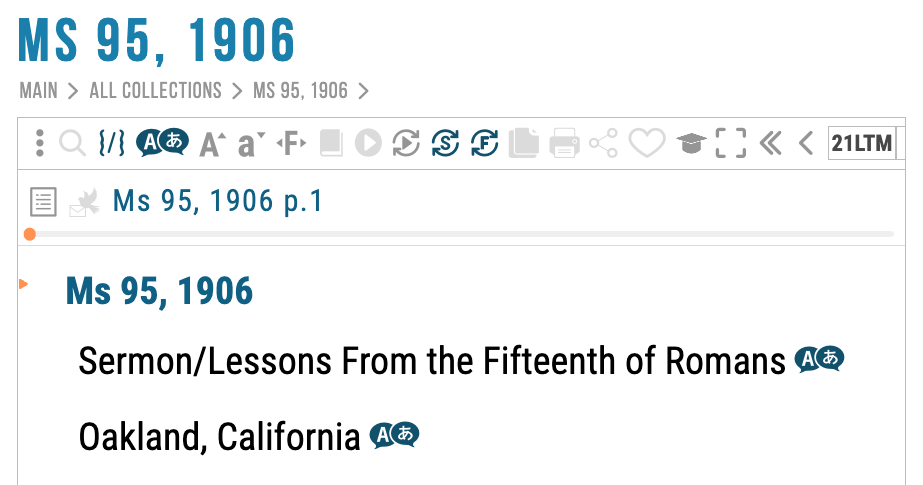
\includegraphics[width=1\linewidth]{images/sermons-and-talks.png}
    \label{fig:enter-label}
\end{figure}


\begin{figure}
    \centering
    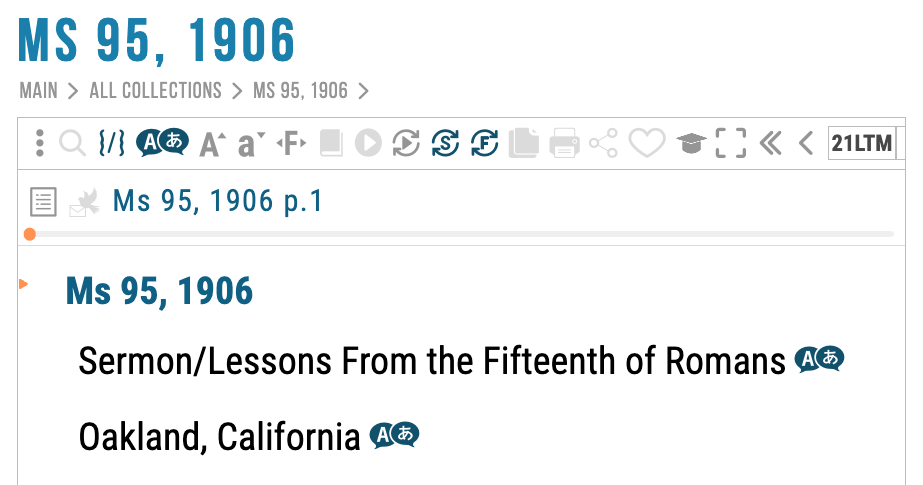
\includegraphics[width=1\linewidth]{images/sermons-and-talks.png}
    \label{fig:enter-label}
\end{figure}


For us, personally, these quotations are unauthenticated and, especially, invalid compared to Ellen White’s authenticated works. But if someone insists on weighing her unconfirmed reports and published writings equally, we will not stand in their way but even further push the conclusion of the Holy Spirit as a being. Let’s follow together.


Para nosotros, personalmente, estas citas no están autenticadas y, especialmente, no son válidas en comparación con las obras autenticadas de Ellen White. Pero si alguien insiste en medir por igual sus informes no confirmados y sus escritos publicados, no nos interpondremos en su camino, sino que impulsaremos aún más la conclusión del Espíritu Santo como un ser. Sigamos juntos.


Even compared with Ellen White’s authenticated works, such a Holy Spirit, a being, would not be one with God because Christ was \egwinline{\textbf{The only being who was one with God}}[Lt121-1897.7; 1897][https://egwwritings.org/read?panels=p7266.13]. This Holy Spirit, a being, could not \egwinline{\textbf{enter into all the counsels and purposes of God}}, because Christ was \egwinline{\textbf{the only being}}[PP 34.1; 1890][https://egwwritings.org/read?panels=p84.75] who could do that. This Being is not to be exalted because \egwinline{\textbf{The Father and the Son \underline{alone} are to be exalted}}[YI, July 7, 1898 par.2.; 1898][https://egwwritings.org/read?panels=p469.2964]. The Holy Spirit, as a being, would not fit in the order of heaven as the third being because Satan was \egwinline{\textbf{next to Christ the most exalted \underline{being}} in the heavenly courts}[RH August 9, 1898, par. 7; 1898][https://egwwritings.org/read?panels=p821.17145]. This Holy Spirit, a being, was not invested in the cost of salvation; neither was he in the covenant with Father and Son to save the world, nor dishonored by man’s transgression.


Incluso comparado con las obras autenticadas de Ellen White, tal Espíritu Santo, un ser, no sería uno con Dios porque Cristo era \egwinline{\textbf{El único ser que era uno con Dios}}[Lt121-1897.7; 1897][https://egwwritings.org/read?panels=p7266.13]. Este Espíritu Santo, un ser, no podría \egwinline{\textbf{entrar en todos los consejos y propósitos de Dios}}, porque Cristo era \egwinline{\textbf{el único ser}}[PP 34.1; 1890][https://egwwritings.org/read?panels=p84.75] que podía hacerlo. Este Ser no debe ser exaltado porque \egwinline{\textbf{El Padre y el Hijo \underline{solamente} deben ser exaltados}}[YI, July 7, 1898 par.2.; 1898][https://egwwritings.org/read?panels=p469.2964]. El Espíritu Santo, como ser, no encajaría en el orden del cielo como el tercer ser porque Satanás era \egwinline{\textbf{junto a Cristo el \underline{ser} más exaltado}} en los atrios celestiales}[RH August 9, 1898, par. 7; 1898][https://egwwritings.org/read?panels=p821.17145]. Este Espíritu Santo, un ser, no fue investido en el costo de la salvación; ni estuvo en la alianza con el Padre y el Hijo para salvar al mundo, ni fue deshonrado por la transgresión del hombre.


\egwinline{The great gift of salvation has been placed within our reach at an \textbf{infinite cost to the Father and the Son}.}[RH November 21, 1912, par. 2; 1912][https://egwwritings.org/read?panels=p821.33329]


\egwinline{El gran don de la salvación ha sido puesto a nuestro alcance a un \textbf{costo infinito para el Padre y el Hijo}.}[RH November 21, 1912, par. 2; 1912][https://egwwritings.org/read?panels=p821.33329]


\egwinline{In the plan to save a lost world, the counsel was between them \textbf{\underline{both}}; \textbf{the covenant of peace was between the Father and the Son}.}[ST December 23, 1897, par. 2; 1897][https://egwwritings.org/read?panels=p820.14803]


\egwinline{En el plan para salvar a un mundo perdido, el consejo fue entre \textbf{\underline{ambos}}; \textbf{el pacto de paz fue entre el Padre y el Hijo}.}[ST December 23, 1897, par. 2; 1897][https://egwwritings.org/read?panels=p820.14803]


\egwinline{But in the transgression of man \textbf{\underline{both} the Father and the Son were dishonored}.}[ST December 12, 1895, par. 7; 1895][https://egwwritings.org/read?panels=p820.13243]


\egwinline{Pero en la transgresión del hombre \textbf{\underline{tanto} el Padre como el Hijo fueron deshonrados}.}[ST December 12, 1895, par. 7; 1895][https://egwwritings.org/read?panels=p820.13243]


Such a Holy Spirit, a being, does not fit into harmony with the authenticated reports of Ellen White, nor with the Scriptures. The Holy Spirit is called ‘\textit{spirit}’, so it is a spirit, exclusively.


Tal Espíritu Santo, un ser, no encaja en armonía con los informes autenticados de Ellen White, ni con las Escrituras. El Espíritu Santo es llamado ‘\textit{espíritu}’, por lo que es un espíritu, exclusivamente.


Many of Sister White’s quotations are sourced from sermons or talks that were published after her death. In what follows, we will present a few that are most often discussed in an effort to prove that Sister White was a trinitarian. We invite everyone to weigh these quotations with her authenticated and published work, those during her lifetime.


Muchas de las citas de la hermana White provienen de sermones o charlas que se publicaron después de su muerte. En lo que sigue, presentaremos algunas de las que más se discuten en un esfuerzo por probar que la hermana White era trinitaria. Invitamos a todos a sopesar estas citas con sus obras autenticadas y publicadas, aquellas durante su vida.


“\textit{And then the golden harps are touched, and the music flows all through the heavenly host, and they fall down and worship the Father and the Son and the Holy Spirit}.”\footnote{\href{https://egwwritings.org/?ref=en_Ms139-1906.32&para=9579.38}{EGW; Ms139-1906.32; 1906}} [Sermon/Thoughts on Matthew 4. Oakland, California July 24, 1906; Previously unpublished.]


“\textit{Y entonces se tocan las arpas de oro, y la música fluye por toda la hueste celestial, y se postran y adoran al Padre y al Hijo y al Espíritu Santo}.”\footnote{\href{https://egwwritings.org/?ref=en_Ms139-1906.32&para=9579.38}{EGW; Ms139-1906.32; 1906}} [Sermón/Thoughts on Matthew 4. Oakland, California 24 de julio de 1906; Previamente inédito.]


“\textit{We need to realize that the Holy Spirit, who is as much a person as God is a person, is walking through these grounds.}”\footnote{\href{https://egwwritings.org/?ref=en_Ms66-1899.11&para=6622.19}{EGW; Ms66-1899.11: 1899}} [Talk/Extracts From Talks Given by Mrs. E. G. White at the Opening of College Hall, Avondale, and in the Avondale Church]


“\textit{Tenemos que darnos cuenta de que el Espíritu Santo, que es tan persona como Dios es persona, está caminando por estos terrenos}.”\footnote{\href{https://egwwritings.org/?ref=en_Ms66-1899.11&para=6622.19}{EGW; Ms66-1899.11: 1899}} [Charla/Extractos de charlas dadas por la Sra. E. G. White en la inauguración de College Hall, Avondale, y en la iglesia de Avondale]
